% ==============================================================================
% AKTIVITETI 01: SFIDA E KAOSIT TË TË DHËNAVE
% AI si Motor Standardizimi
% ==============================================================================
% Kohëzgjatja: 60 minuta
% Audienca: Stafi IT i Gjendjes Civile Shqiptare
% ==============================================================================

\documentclass[aspectratio=169,11pt]{beamer}

% ------------------------------------------------------------------------------
% PAKETAT DHE KONFIGURIMI
% ------------------------------------------------------------------------------
\usepackage[utf8]{inputenc}
\usepackage[T1]{fontenc}
\usepackage[albanian]{babel}
\usepackage{lmodern}
\usepackage{graphicx}
\usepackage{booktabs}
\usepackage{xcolor}
\usepackage{tikz}
\usepackage{fontawesome5}
\usepackage{tcolorbox}
\usepackage{listings}

% Konfigurimi i temës
\usetheme{Madrid}
\usecolortheme{whale}

% Ngjyrat e personalizuara
\definecolor{govblue}{RGB}{0,51,102}
\definecolor{alertred}{RGB}{204,0,0}
\definecolor{successgreen}{RGB}{0,128,0}
\definecolor{warningyellow}{RGB}{255,193,7}

\setbeamercolor{palette primary}{bg=govblue}
\setbeamercolor{frametitle}{bg=govblue,fg=white}

% Hiq simbolet e navigimit
\setbeamertemplate{navigation symbols}{}

% Footer
\setbeamertemplate{footline}[frame number]

% Konfigurimi i listings
\lstset{
  basicstyle=\ttfamily\small,
  breaklines=true,
  frame=single,
  backgroundcolor=\color{gray!10}
}

% ------------------------------------------------------------------------------
% FAQJA E TITULLIT
% ------------------------------------------------------------------------------
\title[Aktiviteti 01]{\textbf{SFIDA E KAOSIT TË TË DHËNAVE}}
\subtitle{AI si Motor Standardizimi}
\author{Workshop: AI dhe Dokumentet Biometrike}
\institute{Dita 1 -- Aktiviteti 1 nga 6}
\date{Kohëzgjatja: 60 minuta}

\begin{document}

% Slide titulli
\begin{frame}
\titlepage
\end{frame}

% ------------------------------------------------------------------------------
% OBJEKTIVAT E TË NXËNIT
% ------------------------------------------------------------------------------
\begin{frame}{Objektivat e të Nxënit}
\vspace{0.5cm}
Në fund të këtij aktiviteti, ju do të jeni në gjendje të:

\vspace{0.5cm}

\begin{enumerate}
    \item \textbf{Përdorni AI për të standardizuar} formate të pakonsisueshme datash në ISO 8601
    \item \textbf{Aplikoni pastrimin me ndihmën e AI} për të normalizuar kapitalizimin e emrave
    \item \textbf{Zbuloni anomali të dhënash} duke përdorur prompt-e validimi AI
    \item \textbf{Dokumentoni prompt-e efektive} për ripërdorim në operacionet e përditshme
\end{enumerate}

\vspace{0.5cm}

\begin{tcolorbox}[colback=warningyellow!20,colframe=warningyellow,title=\faIcon{clock} Shpërndarja e Kohës]
\small
Faza A: Demo Facilitatori (10 min) $\rightarrow$ Faza B: Praktikë e Udhëhequr (40 min) $\rightarrow$ Faza C: Debriefing (10 min)
\end{tcolorbox}

\end{frame}

% ------------------------------------------------------------------------------
% PROBLEMI
% ------------------------------------------------------------------------------
\begin{frame}{Problemi: Kaosi i të Dhënave në Terren}

\begin{columns}
\begin{column}{0.5\textwidth}
\textbf{Realiteti Juaj:}
\begin{itemize}
    \item 50+ rekorde qytetarësh mbërrijnë nga dega rajonale
    \item Datat në 5+ formate të ndryshme
    \item Emrat me kapitalizim rastësor
    \item Adresat të shkurtuara në mënyra të ndryshme
    \item Duhet të futen në bazën e të dhënave SOT
\end{itemize}
\end{column}

\begin{column}{0.5\textwidth}
\begin{tcolorbox}[colback=alertred!10,colframe=alertred,title=\faIcon{exclamation-triangle} Shembull Kaosi]
\small
\texttt{15/03/1987}\\
\texttt{Mars 15, 1987}\\
\texttt{1987-03-15}\\
\texttt{15 Mars 1987}\\
\texttt{870315}
\end{tcolorbox}

\vspace{0.3cm}

\textbf{Të gjitha përfaqësojnë TË NJËJTËN datë!}
\end{column}
\end{columns}

\end{frame}

% ------------------------------------------------------------------------------
% ZGJIDHJA
% ------------------------------------------------------------------------------
\begin{frame}{Zgjidhja: AI si Motori Juaj i Standardizimit}

\begin{center}
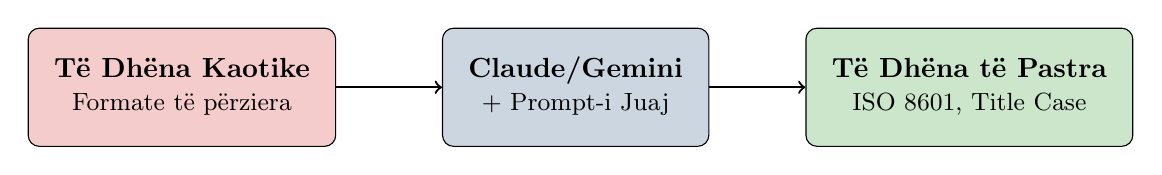
\begin{tikzpicture}
    % Kutia input
    \node[draw, fill=alertred!20, minimum width=3cm, minimum height=1.5cm, rounded corners] (input) at (0,0) {
        \begin{tabular}{c}
        \textbf{Të Dhëna Kaotike}\\
        \small Formate të përziera
        \end{tabular}
    };
    
    % Kutia AI
    \node[draw, fill=govblue!20, minimum width=3cm, minimum height=1.5cm, rounded corners] (ai) at (5,0) {
        \begin{tabular}{c}
        \textbf{Claude/Gemini}\\
        \small + Prompt-i Juaj
        \end{tabular}
    };
    
    % Kutia output
    \node[draw, fill=successgreen!20, minimum width=3cm, minimum height=1.5cm, rounded corners] (output) at (10,0) {
        \begin{tabular}{c}
        \textbf{Të Dhëna të Pastra}\\
        \small ISO 8601, Title Case
        \end{tabular}
    };
    
    % Shigjetat
    \draw[->, thick] (input) -- (ai);
    \draw[->, thick] (ai) -- (output);
\end{tikzpicture}
\end{center}

\vspace{0.5cm}

\begin{tcolorbox}[colback=successgreen!10,colframe=successgreen,title=\faIcon{check-circle} Pikëpamja Kyçe]
AI shkëlqen në \textbf{detyrat e përsëritura të standardizimit} që do t'u merrnin njerëzve orë të tëra. Detyra juaj është të hartoni udhëzimet e duhura (prompt-et).
\end{tcolorbox}

\end{frame}

% ------------------------------------------------------------------------------
% STANDARDET E SYNUARA
% ------------------------------------------------------------------------------
\begin{frame}{Standardet e Synuara për Regjistrin Civil Shqiptar}

\begin{tabular}{lll}
\toprule
\textbf{Fusha} & \textbf{Shembull Kaotik} & \textbf{Formati i Standardizuar} \\
\midrule
Datëlindja & 15/03/1987 & \textcolor{successgreen}{1987-03-15} (ISO 8601) \\
Emri i Plotë & agron HOXHA & \textcolor{successgreen}{Agron Hoxha} (Title Case) \\
Gjinia & mashkull, Male, m & \textcolor{successgreen}{M} (Shkronjë e vetme) \\
Telefoni & 0682345678 & \textcolor{successgreen}{+355682345678} (E.164) \\
\bottomrule
\end{tabular}

\vspace{0.5cm}

\begin{tcolorbox}[colback=govblue!10,colframe=govblue,title=\faIcon{info-circle} Pse ISO 8601?]
\small
Standardi ndërkombëtar eliminon paqartësinë: A është 03/04/2024 4 Mars apo 3 Prill? \\
Formati ISO 8601 \texttt{VVVV-MM-DD} është i qartë dhe renditet kronologjikisht.
\end{tcolorbox}

\end{frame}

% ------------------------------------------------------------------------------
% DEMO: HARTIMI I PROMPT-IT
% ------------------------------------------------------------------------------
\begin{frame}[fragile]{Demo: Hartimi i Prompt-it Tuaj të Standardizimit}

\begin{tcolorbox}[colback=gray!10,colframe=gray,title=\faIcon{robot} Shembull Prompt-i për Claude/Gemini]
\small
\begin{verbatim}
Kam një skedar CSV me rekorde qytetarësh shqiptarë.
Të dhënat kanë formatim të pakonsisueshëm.

Ju lutem standardizoni sa më poshtë:

1. Konvertoni TË GJITHA datat në formatin ISO 8601 (VVVV-MM-DD)
2. Konvertoni TË GJITHA emrat në Title Case (Agron Hoxha)
3. Konvertoni gjininë në shkronjë të vetme (M ose F)
4. Sinjalizoni çdo rekord me:
   - Datëlindje në të ardhmen (e pamundur)
   - Moshë mbi 120 vjet (e pabesueshme)
   - Fusha të detyrueshme që mungojnë

Rezultati si CSV i pastër me kolonë shënime_validimi.
\end{verbatim}
\end{tcolorbox}

\end{frame}

% ------------------------------------------------------------------------------
% DETYRA JUAJ
% ------------------------------------------------------------------------------
\begin{frame}{Detyra Juaj (40 Minuta)}

\begin{enumerate}
    \item \textbf{Hapni} \texttt{rekordet\_qytetareve\_kaotike.csv} në menaxherin e skedarëve
    
    \item \textbf{Ngarkoni} skedarin në Claude ose Gemini
    
    \item \textbf{Shkruani prompt-e} për të:
    \begin{itemize}
        \item Konvertuar datat në ISO 8601
        \item Standardizuar emrat në Title Case
        \item Normalizuar kodet e gjinisë
        \item Sinjalizuar rekorde anomale
    \end{itemize}
    
    \item \textbf{Eksportoni} datasetin tuaj të pastruar
    
    \item \textbf{Sfidë Bonus:} Gjeni 3 anomalitë e fshehura!
\end{enumerate}

\vspace{0.3cm}

\begin{tcolorbox}[colback=warningyellow!20,colframe=warningyellow,title=\faIcon{trophy} Konkursi]
Pjesëmarrësi i parë që identifikon saktësisht të 3 anomalitë fiton një çmim!
\end{tcolorbox}

\end{frame}

% ------------------------------------------------------------------------------
% TIPET E ANOMALIVE
% ------------------------------------------------------------------------------
\begin{frame}{Tipet e Anomalive për t'u Zbuluar}

Dataseti përmban 3 gabime të fshehura që AI duhet t'i sinjalizojë:

\vspace{0.5cm}

\begin{tabular}{cl}
\faIcon{calendar-times} & \textbf{Tipi 1:} Datëlindje në TË ARDHMEN (e pamundur) \\
\\
\faIcon{user-clock} & \textbf{Tipi 2:} Mosha mbi 120 vjet (e pabesueshme) \\
\\
\faIcon{id-card} & \textbf{Tipi 3:} NID nuk përputhet me modelin e datëlindjes \\
\end{tabular}

\vspace{0.5cm}

\begin{tcolorbox}[colback=govblue!10,colframe=govblue,title=\faIcon{lightbulb} Këshillë Prompt-i]
Pyesni AI: ``Për çdo rekord, verifikoni që datëlindja rezulton në një moshë të vlefshme ndërmjet 0 dhe 120 vjet. Sinjalizoni çdo rekord jashtë këtij diapazoni.''
\end{tcolorbox}

\end{frame}

% ------------------------------------------------------------------------------
% KËSHILLA PËR RAFINIM PROMPT-I
% ------------------------------------------------------------------------------
\begin{frame}{Këshilla për Rafinimin e Prompt-eve}

\begin{columns}
\begin{column}{0.5\textwidth}
\textbf{\textcolor{alertred}{\faIcon{times-circle} Prompt i Dobët:}}
\begin{tcolorbox}[colback=alertred!10,colframe=alertred]
\small
``Pastro këto të dhëna''
\end{tcolorbox}

\vspace{0.3cm}
\textit{Shumë i paqartë -- AI nuk di standardet tuaja}
\end{column}

\begin{column}{0.5\textwidth}
\textbf{\textcolor{successgreen}{\faIcon{check-circle} Prompt i Fortë:}}
\begin{tcolorbox}[colback=successgreen!10,colframe=successgreen]
\small
``Konverto kolonën datëlindja në ISO 8601 (VVVV-MM-DD). Formatet input mund të përfshijnë DD/MM/VVVV, Muaji DD VVVV, ose DD Muaji VVVV.''
\end{tcolorbox}

\vspace{0.3cm}
\textit{Format specifik + shembuj = rezultate më të mira}
\end{column}
\end{columns}

\vspace{0.5cm}

\textbf{Receta për Prompt-e të Mirë:}
\begin{enumerate}
    \item Deklaroni \textbf{formatin input} (çfarë keni)
    \item Deklaroni \textbf{formatin output} (çfarë ju nevojitet)
    \item Jepni \textbf{shembuj} të rasteve kufitare
    \item Specifikoni sjelljen e \textbf{trajtimit të gabimeve}
\end{enumerate}

\end{frame}

% ------------------------------------------------------------------------------
% DISKUTIMI I DEBRIEFING-UT
% ------------------------------------------------------------------------------
\begin{frame}{Diskutimi i Debriefing-ut (10 Minuta)}

\begin{enumerate}
    \item \textbf{Cilat formulime prompt-esh} prodhuan rezultatin më të pastër?
    
    \vspace{0.3cm}
    
    \item \textbf{A i kapi AI} të tri anomalitë e vendosura? Cilat i humbi?
    
    \vspace{0.3cm}
    
    \item \textbf{Si do ta integronit} këtë rrjedhë pune në procesin tuaj të përditshëm të futjes së të dhënave?
    
    \vspace{0.3cm}
    
    \item \textbf{Cilat raste kufitare} do t'ju duhej të trajtonit për të dhëna reale shqiptare?
\end{enumerate}

\vspace{0.5cm}

\begin{tcolorbox}[colback=govblue!10,colframe=govblue,title=\faIcon{save} Veprim]
Dokumentoni prompt-in tuaj më efektiv në Bibliotekën Tuaj Personale të Prompt-eve (Aktiviteti 6)
\end{tcolorbox}

\end{frame}

% ------------------------------------------------------------------------------
% PIKAT KYÇE
% ------------------------------------------------------------------------------
\begin{frame}{Pikat Kyçe}

\begin{enumerate}
    \item \faIcon{robot} \textbf{AI si mjet përputhshmërie:} Zbaton standarde në mënyrë konsistente në shkallë
    
    \vspace{0.3cm}
    
    \item \faIcon{calendar-check} \textbf{ISO 8601:} Standardi ndërkombëtar i datës (VVVV-MM-DD)
    
    \vspace{0.3cm}
    
    \item \faIcon{edit} \textbf{Inxhinieria e prompt-eve:} Udhëzime specifike japin rezultate specifike
    
    \vspace{0.3cm}
    
    \item \faIcon{exclamation-triangle} \textbf{Zbulimi i anomalive:} AI mund të sinjalizojë automatikisht të dhëna të pamundura
\end{enumerate}

\vspace{0.5cm}

\begin{center}
\Large
\textbf{Në vazhdim: Aktiviteti 2 -- Validuesi i të Dhënave ICAO 9303}
\end{center}

\end{frame}

\end{document}

